%!TEX root = ../../main.tex

\subsection{Sensoroe BDD}

\begin{figure}[H]
	\centering
	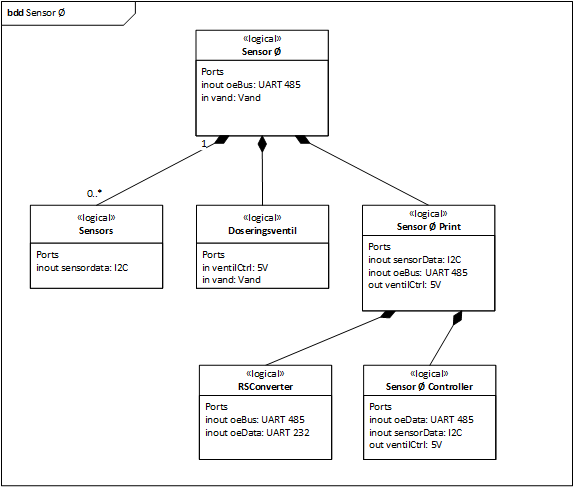
\includegraphics[width=0.82\textwidth]{Systemarkitektur/Sensoroe/Sensoroe_BDD.png}
	\label{fig:Sensoroe BDD}
	\caption{Block Definition Diagram af Sensoroe}
\end{figure}

\subsubsection*{Sensor Ø Control}
Sensor Ø Control tager imod kommandoer fra KarControl, som instruerer omkring åbning og lukning af Doseringsventil. KarControl anmoder også om, at Sensor Ø Control skal sende måledata fra sensors, som er tilkoblet Sensor Ø’en.

\subsubsection{Doseringsventil}
Doseringsventilen åbner og lukker for vandtilførslen til planterne i området omkring Sensor Ø’en, som Doseringsventilen er tilkoblet. Når KarControl tænder for Vandpumpen kan de enkelte Sensor Ø’ers Doseringsventiler være åbne eller lukkede alt efter, om planterne omkring Sensor Ø’en har brug for vand.

\subsubsection{Sensor}
Sensor er en generalisering af alle slags sensorer, som kan tilsluttes Sensor Ø’en. Vilkårligt mange sensorer kan tilkobles en bus, og kommunikere med Sensor Ø Control gennem en standardiseret protokol. Sensor kan kun aflevere målinger når de bliver bedt om at levere dem.

\subsection{Sensoroe IBD}

\begin{figure}[H]
	\centering
	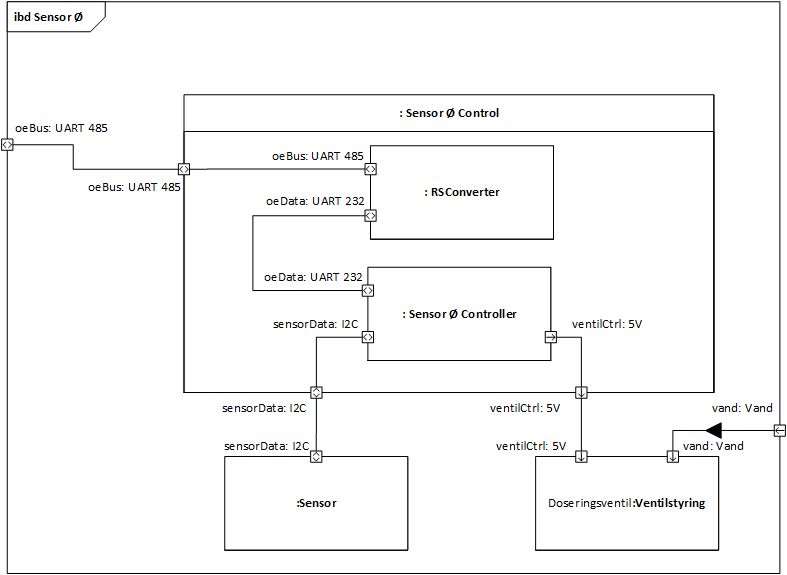
\includegraphics[width=0.82\textwidth]{Systemarkitektur/Sensoroe/Sensoroe_IBD.png}
	\label{fig:Sensoroe BDD}
	\caption{Internal Block Diagram af Sensoroe}
\end{figure}



\subsection{Sensoroe Allokeringsdiagram}

\begin{figure}[H]
	\centering
	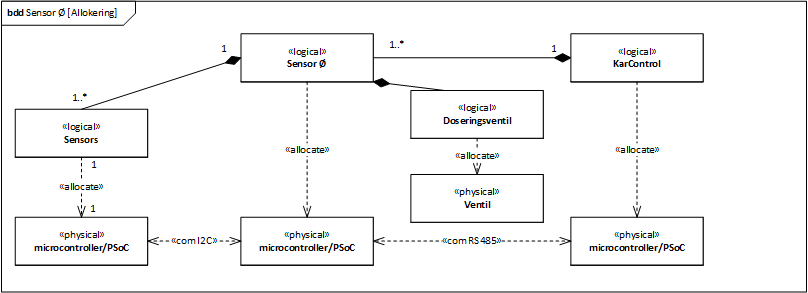
\includegraphics[width=0.82\textwidth]{Systemarkitektur/Sensoroe/Sensoroe_Allokeringsdiagram.png}
	\label{fig:Sensoroe BDD}
	\caption{Allokeringsdiagram af Sensoroe}
\end{figure}